\section{Marco conceptual}

Este marco no es un catálogo de definiciones. Es una construcción de decisiones: qué tipo de tareas importan para aprendizaje profundo, qué teorías orientan cómo pensamos sobre esas tareas, y cómo la IA puede posicionarse pedagógicamente para expandir —nunca reemplazar— la actividad matemática del estudiante. Las secciones que siguen desarrollan los fundamentos que articulan el diseño de la investigación.

% ─────────────────────────────────────────────────────────────
\subsection{Ejercicio versus tarea: diferencia operativa}
% ─────────────────────────────────────────────────────────────

En las aulas se usa la palabra ``tarea'' para casi cualquier cosa que se pide. Pero esta investigación trabaja con una distinción específica. No es semántica. Es conceptual.

Un \textbf{ejercicio}: el estudiante aplica un procedimiento conocido a situaciones similares. Ejemplo: ``Calcula $\mathrm{sen}(45°)$'' o ``Resuelve $2\mathrm{sen}(x) = 1$ donde $x \in [0, 2\pi]$''. Tiene valor: consolida destreza. Pero encierra el pensamiento. El estudiante reconoce qué fórmula aplicar, hace los pasos, obtiene respuesta. Eso es automatización de procedimientos. No necesariamente comprensión conceptual profunda.

Una \textbf{tarea}: requiere exploración. Ejemplo: ``Un arquitecto diseña una rampa de acceso con ángulo máximo de $30°$. El espacio vertical disponible es 1{,}5 metros. ¿Cuál es la longitud mínima de la rampa? Dibuja la situación, justifica qué razón trigonométrica usaste y explica por qué tu respuesta tiene sentido en contexto.'' Aquí el estudiante no puede simplemente reconocer y aplicar una fórmula. Necesita interpretar contexto, decidir qué representación elegir (dibujo, ecuación, tabla), coordinar conceptos (ángulo, distancia, relación trigonométrica) y justificar la decisión. Exige pensamiento genuino \parencite{leungDesigningMathematicsTasks2015, radmehrTheoreticalFrameworkTask2023, canogullariTaskDesignPrinciples2025}.

Esta distinción orienta el diseño de la investigación: las actividades propuestas no son ejercicios. Son problemas auténticos que requieren razonamiento trigonométrico real.

% ─────────────────────────────────────────────────────────────
\subsection{La trigonometría: recorrido histórico y currículo colombiano}
% ─────────────────────────────────────────────────────────────

\subsubsection{De razón geométrica a función matemática}

La trigonometría no siempre fue lo que es hoy. Su historia es el recorrido de un concepto que nació como herramienta de medición geométrica y se transformó paulatinamente en una familia de funciones matemáticas con dominio en los reales. Comprender ese recorrido ilumina directamente por qué los estudiantes tienen dificultades con la trigonometría escolar: la mayoría de los obstáculos conceptuales que enfrentan hoy son los mismos que la disciplina tuvo que superar históricamente.

En la tradición griega clásica, Hiparco (siglo II a.C.) y Ptolomeo (siglo II d.C.) desarrollaron tablas de cuerdas —no de senos— para calcular posiciones astronómicas. La unidad de medida era la cuerda de un arco en un círculo, no una razón entre lados de un triángulo. La matemática india del siglo V, con Aryabhata, introdujo la \emph{ardha-jya} (semiacuerda), concepto más cercano al seno moderno, que los matemáticos árabes medievales tradujeron y transmitieron a Europa bajo el nombre \emph{sinus} \parencite[p.~311]{katzCalculusTrigonometricFunctions1987}.

El salto conceptual decisivo ocurrió en el siglo XVIII con Euler, quien redefinió las funciones trigonométricas no como razones geométricas sino como funciones de variable real asociadas al círculo unitario. Con Euler, $\mathrm{sen}(x)$ dejó de ser ``el cateto opuesto sobre la hipotenusa en un triángulo rectángulo'' para convertirse en la coordenada $y$ del punto del círculo unitario determinado por el ángulo $x$. Esa redefinición abrió la puerta a tratar las funciones trigonométricas con las herramientas del análisis: derivadas, integrales, series de potencias, extensión a los complejos \parencite{maorTrigonometricDelights1998}.

Esta historia no es anecdótica. El currículo escolar tiende a replicar la trayectoria histórica: primero razones en triángulo rectángulo, luego extensión al círculo unitario, luego funciones periódicas en el plano cartesiano. Cada transición exige del estudiante una reestructuración conceptual —y es en esas transiciones donde emergen los obstáculos más persistentes. Saber que esos obstáculos también marcaron el desarrollo histórico de la disciplina ayuda al docente a anticiparlos en lugar de sorprenderse ante ellos.

La Figura~\ref{fig:circulo_unitario} muestra la relación fundamental que articula las tres fases del desarrollo conceptual: el seno y el coseno como coordenadas del punto $P$ en el círculo unitario para un ángulo $\theta$.

\begin{figure}[H]
\centering
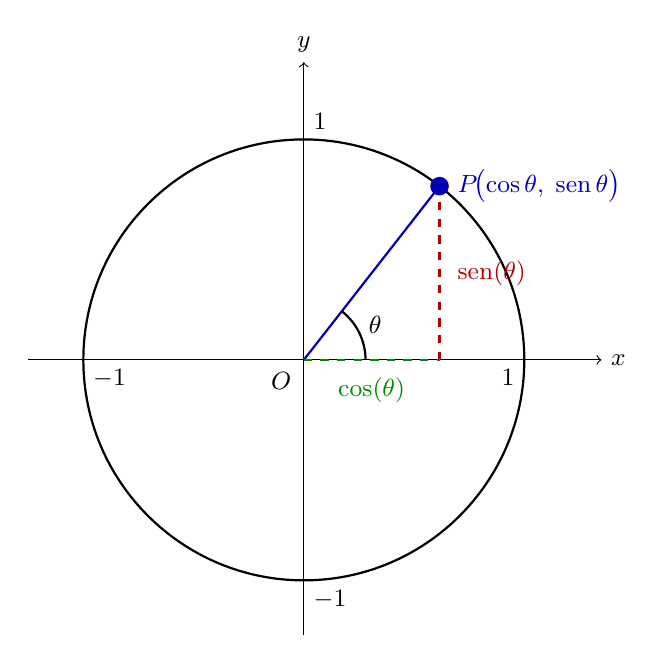
\begin{tikzpicture}[scale=2.8, font=\small]
  % Ejes
  \draw[->] (-1.25,0) -- (1.35,0) node[right] {$x$};
  \draw[->] (0,-1.25) -- (0,1.35) node[above] {$y$};
  % Círculo unitario
  \draw[thick] (0,0) circle (1);
  % Ángulo y radio
  \def\ang{52}
  \draw[thick, blue!70!black] (0,0) -- ({cos(\ang)},{sin(\ang)});
  % Proyecciones
  \draw[dashed, red!70!black, thick] ({cos(\ang)},0) -- ({cos(\ang)},{sin(\ang)});
  \draw[dashed, green!55!black, thick] (0,0) -- ({cos(\ang)},0);
  % Arco del ángulo
  \draw[thick] (0.28,0) arc (0:\ang:0.28);
  \node at ({0.36*cos(\ang/2)},{0.36*sin(\ang/2)}) {$\theta$};
  % Punto P
  \fill[blue!70!black] ({cos(\ang)},{sin(\ang)}) circle (1.2pt);
  \node[right=3pt, blue!70!black] at ({cos(\ang)},{sin(\ang)})
    {$P\!\bigl(\cos\theta,\;\mathrm{sen}\,\theta\bigr)$};
  % Etiquetas proyecciones
  \node[red!70!black, right=3pt] at ({cos(\ang)}, {sin(\ang)/2})
    {$\mathrm{sen}(\theta)$};
  \node[green!55!black, below=3pt] at ({cos(\ang)/2}, 0)
    {$\cos(\theta)$};
  % Marcas de escala
  \foreach \v in {-1,1} {
    \draw (\v, 1.5pt) -- (\v,-1.5pt);
    \draw (1.5pt,\v) -- (-1.5pt,\v);
  }
  \node[below left] at (1,0) {$1$};
  \node[below right] at (-1,0) {$-1$};
  \node[above right] at (0,1) {$1$};
  \node[below right] at (0,-1) {$-1$};
  \node[below left=1pt] at (0,0) {$O$};
\end{tikzpicture}
\caption{Círculo unitario: el seno y el coseno como coordenadas del punto $P$ para el ángulo $\theta$.
La extensión de razón en triángulo rectángulo a coordenada en círculo unitario es el paso conceptual
central que articula el currículo de trigonometría en educación media. Elaboración propia.}
\label{fig:circulo_unitario}
\end{figure}

\subsubsection{La trigonometría en el currículo colombiano}

El currículo colombiano de matemáticas ha evolucionado de forma continua en los últimos treinta años, y esa evolución tiene consecuencias directas para la enseñanza de la trigonometría. No se trata solo de qué contenidos se incluyen, sino de qué tipo de razonamiento se espera que los estudiantes desarrollen y con qué propósito.

Los \emph{Lineamientos Curriculares} \parencite{ministeriodeeducacionnacionalLineamientosCurriculares1998} establecieron el \emph{pensamiento variacional} como uno de los cinco tipos de pensamiento matemático que los estudiantes colombianos deben desarrollar a lo largo de su escolaridad. Dentro de ese pensamiento, las funciones trigonométricas ocupan un lugar central: son el ejemplo canónico de función que describe variación periódica, y su comprensión exige exactamente la articulación entre representación gráfica, algebraica, numérica y contextual que los lineamientos proponen. Esta fue una decisión curricular significativa: posicionó la trigonometría no como técnica de cálculo aislada sino como parte de un programa más amplio de comprensión de la variación matemática.

Los \emph{Estándares Básicos de Competencias} \parencite{ministeriodeeducacionnacionalEstandaresBasicos2006} precisaron ese propósito en estándares observables para los grados décimo y undécimo. Entre ellos: ``Describo y modelo fenómenos periódicos del mundo real usando funciones trigonométricas''. Ese estándar conecta la trigonometría con el mundo real —mareas, movimiento circular, variación térmica— y exige que el estudiante no solo calcule sino que \emph{interprete} y \emph{justifique}. Es el tipo de competencia que no puede evaluarse con un ejercicio rutinario.

Los \emph{Derechos Básicos de Aprendizaje} (DBA) \parencite{ministeriodeeducacionnacionalDerechosBasicos2016} para el grado décimo precisan los aprendizajes concretos esperados: reconocer la amplitud, el período y el desplazamiento de fase de una función trigonométrica; interpretar esos parámetros en contexto; usar el modelo para hacer predicciones verificables. Esos aprendizajes son exactamente los que las dos tareas diseñadas en esta investigación buscan desarrollar y documentar.

Sin embargo, hay una brecha documentada entre lo que el currículo prescribe y lo que ocurre en las aulas. La enseñanza efectiva de la trigonometría en Colombia sigue anclada con frecuencia al procedimiento de razones en triángulos rectángulos, sin alcanzar el nivel funcional y de modelación que los documentos curriculares proponen \parencite{montiel-espinosaDesarrolloPensamientoTrigonometrico2013}. Cerrar esa brecha —diseñando tareas que hagan posible el nivel de pensamiento que el currículo exige— es uno de los propósitos centrales de esta investigación.

% ─────────────────────────────────────────────────────────────
\subsection{Pensamiento trigonométrico}
% ─────────────────────────────────────────────────────────────

Es posible resolver ejercicios de trigonometría sin pensar realmente en trigonometría \parencite{montiel-espinosaDesarrolloPensamientoTrigonometrico2013}. Un estudiante aplica fórmulas, manipula ecuaciones, obtiene respuestas correctas, y aún así no comprende qué representa un seno o coseno más allá de una razón en triángulo rectángulo. El pensamiento trigonométrico genuino va más allá.

Para esta investigación, el pensamiento trigonométrico emerge cuando el estudiante:

\textbf{Primero}, interpreta funciones trigonométricas como objetos funcionales. No como procedimientos (``seno es cateto opuesto sobre hipotenusa''), sino como funciones que describen variación periódica. Significa entender que $y = \mathrm{sen}(x)$ es una relación donde $x$ (el ángulo) es variable independiente e $y$ depende de $x$. Cuando grafica esa relación, ve cómo cambia, interpreta dominio y rango, comprende por qué se repite. Eso es pensamiento funcional sobre trigonometría.

\textbf{Segundo}, articula múltiples representaciones. Una función trigonométrica puede expresarse algebraicamente (ecuación como $y = 2\,\mathrm{sen}(x - \pi/4) + 1$), gráficamente (como curva en el plano), numéricamente (tabla de valores) y verbalmente (``temperatura oscila alrededor de 20°C con amplitud 5° y período 24 horas''). Un estudiante con pensamiento trigonométrico genuino no se queda en un único registro. Puede traducir entre ellos, explicar por qué cada representación resalta aspectos diferentes, usar cada una según el propósito. Esa coordinación requiere esfuerzo y no ocurre espontáneamente \parencite{duval2006}.

\textbf{Tercero}, razona sobre variación y periodicidad con significado. Cuando un problema dice ``función tiene amplitud 3 y período $\pi/2$'', un estudiante sin pensamiento trigonométrico repite palabras sin interpretarlas. Un estudiante con pensamiento trigonométrico explica: amplitud 3 significa oscilación entre $-3$ y $3$; período $\pi/2$ significa que la función completa un ciclo cada $\pi/2$ unidades. Cuando el contexto lo pide, conecta: si el período es $\pi/2$ y representa tiempo en horas, el fenómeno se repite cada $\pi/2$ horas.

\textbf{Cuarto}, diferencia y elige adecuadamente entre radianes y grados. Sabe que ambos son sistemas de medida angular. Entiende que los radianes miden el ángulo en términos del arco en el círculo unitario, mientras los grados dividen el círculo en 360 partes arbitrarias. Cuando trabaja con funciones trigonométricas —donde radianes son el sistema estándar del análisis matemático—, los usa. Cuando el contexto lo requiere, convierte. Esa flexibilidad es signo de pensamiento conceptual.

\textbf{Quinto}, argumenta matemáticamente sobre situaciones problemáticas. No solo resuelve. Además explica por qué su método funciona, qué supuestos hizo, cuáles serían las limitaciones si las condiciones cambiaran, cómo sabe que la respuesta tiene sentido \parencite{montiel-espinosaDesarrolloPensamientoTrigonometrico2013}.

Estas cinco características no son abstractas. Son observables en el aula cuando un estudiante resuelve una tarea: en cómo dibuja la situación, qué expresa algebraicamente, cómo explica sus decisiones, cómo valida la respuesta.

% ─────────────────────────────────────────────────────────────
\subsection{Desarrollo escolar de funciones trigonométricas}
% ─────────────────────────────────────────────────────────────

Las funciones trigonométricas tienen una estructura lógica donde algunas ideas deben preceder a otras \parencite{hsuReviewMathematicalTasks2023}.

Para esta investigación, el desarrollo se estructura en tres fases conectadas, cuya articulación se ilustra en la Figura~\ref{fig:funcion_seno}.

\textbf{Primera fase}: la razón trigonométrica en triángulo rectángulo como fundación. Un estudiante que comprende que en un triángulo rectángulo el seno de un ángulo es la razón entre cateto opuesto e hipotenusa tiene una base. Pero esa base es limitada: funciona solo con ángulos agudos, solo en triángulos rectángulos. El objetivo es que el estudiante sea consciente de esa limitación.

\textbf{Segunda fase}: extensión del concepto al círculo unitario. El triángulo rectángulo entra en un círculo. El ángulo ya no está restringido; puede ser cualquier valor real. La hipotenusa siempre mide 1 (por eso ``unitario''). Ahora el seno de cualquier ángulo es la coordenada $y$ del punto donde el lado terminal del ángulo intersecta el círculo. Eso es crucial: seno deja de ser solo razón y empieza a ser coordenada. La interpretación cambia.

\textbf{Tercera fase}: funciones trigonométricas en el plano cartesiano. Si varío el ángulo de forma continua y trazo los puntos $(x,\, \mathrm{sen}(x))$, obtengo una curva. Esa curva es periódica, oscila, tiene amplitud y período. Se pasa de punto a curva, de valor aislado a función, de estática a variación continua. Los parámetros $A$, $B$, $C$ y $D$ en la expresión $y = A\,\mathrm{sen}(Bx + C) + D$ tienen significado geométrico y contextual preciso.

Estos tres niveles no deben enseñarse desconectados. Un estudiante que ve triángulos rectángulos durante semanas, luego salta al círculo unitario, luego a gráficas, experimentará rupturas conceptuales. Las tareas deben diseñarse para conectar esos niveles, mostrando cómo la razón en triángulo se extiende a coordenada en círculo y luego a función continua en el plano \parencite{montiel-espinosaDesarrolloPensamientoTrigonometrico2013}.

\begin{figure}[H]
\centering
\begin{tikzpicture}
\begin{axis}[
  width=13cm, height=6.5cm,
  axis lines=center,
  xlabel={$x$},
  ylabel={$y$},
  xlabel style={at={(ticklabel* cs:1)}, anchor=west},
  ylabel style={at={(ticklabel* cs:1)}, anchor=south},
  xmin=-0.4, xmax=13.5,
  ymin=-3.8, ymax=4.5,
  xtick={1.5708, 3.1416, 4.7124, 6.2832, 7.8540, 9.4248, 10.9956, 12.5664},
  xticklabels={$\frac{\pi}{2}$, $\pi$, $\frac{3\pi}{2}$, $2\pi$,
               $\frac{5\pi}{2}$, $3\pi$, $\frac{7\pi}{2}$, $4\pi$},
  ytick={-3,-2,-1,1,2,3},
  samples=300,
  smooth,
  tick label style={font=\small},
  label style={font=\small},
  grid=none,
]
  % Línea central D
  \addplot[gray!50, dashed, thick, domain=-0.3:13.3] {0.5};

  % Función y = 2.5·sen(x) + 0.5
  \addplot[blue!70!black, very thick, domain=0:12.8] {2.5*sin(deg(x))+0.5};

  % Anotaciones de amplitud
  \draw[<->, red!70!black, thick]
    (axis cs:1.5708, 0.5) -- (axis cs:1.5708, 3.0)
    node[midway, right=3pt, font=\small] {$A$};

  % Anotación del período
  \draw[<->, green!50!black, thick]
    (axis cs:0.0, -3.5) -- (axis cs:6.2832, -3.5)
    node[midway, below=3pt, font=\small] {$T = \dfrac{2\pi}{B}$};

  % Etiqueta D
  \node[gray!70!black, right=2pt, font=\small] at (axis cs:13.0, 0.5) {$D$};

  % Etiqueta función
  \node[blue!70!black, font=\small] at (axis cs:9.8, 3.4)
    {$y = A\,\mathrm{sen}(Bx + C) + D$};
\end{axis}
\end{tikzpicture}
\caption{Función $y = A\,\mathrm{sen}(Bx + C) + D$ con sus parámetros fundamentales.
La amplitud $A$ determina la magnitud de la oscilación respecto a la línea media $D$;
el período $T = 2\pi/B$ determina la longitud del ciclo completo;
el desfase $C$ desplaza horizontalmente la función.
Comprender el significado contextual de cada parámetro es el objetivo central
de las tareas de esta investigación. Elaboración propia.}
\label{fig:funcion_seno}
\end{figure}

% ─────────────────────────────────────────────────────────────
\subsection{Errores y obstáculos}
% ─────────────────────────────────────────────────────────────

\textcite{brousseauTheoryDidacticalSituations2002} acuñó el término \emph{obstáculo epistemológico} para describir errores que no son meras faltas de atención sino que surgen de una comprensión incompleta que el estudiante debe superar activamente. En trigonometría, estos obstáculos son reales y documentados.

Cuando un estudiante confunde razón con función, ese error no es casualidad. Surge porque está aplicando una interpretación que funciona en el contexto restringido del triángulo rectángulo pero no en el contexto ampliado de las funciones periódicas. El error es una manifestación de que el estudiante todavía no ha integrado los dos marcos conceptuales. Cuando el error se hace visible en una tarea, se discute, y se contrasta con estrategias alternativas que sí funcionan en el contexto general, hay oportunidad de que el estudiante reestructure su comprensión.

Si el error se oculta o se penaliza sin discusión, el estudiante lo repite. La investigación en educación matemática es consistente al respecto \parencite{brousseauTheoryDidacticalSituations2002, arhinAnalysisHighSchool2021}: los errores gestionados productivamente son oportunidades de aprendizaje más valiosas que respuestas correctas acríticas.

Los obstáculos más documentados en trigonometría escolar son:

\begin{itemize}
\item \textbf{Confusión razón–función:} el estudiante aplica $\mathrm{sen}(\theta) = \text{CO}/\text{H}$ en contextos donde la función trigonométrica describe variación continua, no una razón fija en un triángulo específico.
\item \textbf{Interpretación incorrecta de la amplitud:} confundir el valor máximo de la función con la amplitud, o no reconocer la amplitud como la distancia entre el valor máximo y la línea media.
\item \textbf{Errores en el período:} confundir el coeficiente $B$ directamente con el período, sin aplicar la relación $T = 2\pi/B$.
\item \textbf{Dificultades con los radianes:} operar mecánicamente entre grados y radianes sin comprender que son dos formas de medir el mismo ángulo.
\item \textbf{Desconexión parámetro–contexto:} calcular correctamente los parámetros de una función sin poder interpretar qué significan en la situación física que modelan.
\end{itemize}

Las tareas de esta investigación están diseñadas para hacer visibles estos obstáculos. No para evitarlos, sino para provocar que emerjan y puedan ser examinados \parencite{leungDesigningMathematicsTasks2015}.

% ─────────────────────────────────────────────────────────────
\subsection{GeoGebra y génesis instrumental}
% ─────────────────────────────────────────────────────────────

Durante décadas, la matemática se enseñó con papel y pizarrón. El estudiante llenaba cuadernos con gráficas trazadas a mano, cálculos mecánicos, ecuaciones copiadas. Las herramientas como GeoGebra transforman esa experiencia de forma fundamental: no son simplemente un crayón digital. Cuando un estudiante mueve un deslizador que controla la amplitud de una función seno, la gráfica responde en tiempo real. Ve que amplitud 2 produce una oscilación entre $-2$ y $2$, que amplitud 5 la extiende entre $-5$ y $5$. No memorizado. Visto. Experimentado. \parencite{hohenwartherCombinationDynamicGeometry2004, zenginEffectDynamicMathematics2012}.

Sin embargo, la mera disponibilidad de una herramienta potente no garantiza aprendizaje. \textcite{troucheManagingComplexityHuman2004} desarrolló el concepto de \emph{génesis instrumental} para distinguir entre un \emph{artefacto} (el software tal como existe, independientemente del usuario) y un \emph{instrumento} (el artefacto integrado en la actividad del sujeto a través del uso). GeoGebra no es automáticamente un instrumento para quien lo usa por primera vez. Se convierte en instrumento en la medida en que el estudiante desarrolla esquemas de uso: sabe qué herramientas usar para qué propósito, cómo interpretar los resultados, cuándo confiar en la representación gráfica y cuándo el cálculo algebraico es más preciso.

Esta distinción tiene implicaciones directas para el diseño de las tareas. Una tarea que pide ``grafica la función que el docente dicta en GeoGebra'' mantiene a los estudiantes en el nivel del artefacto: usan el software mecánicamente, sin desarrollar comprensión sobre lo que están representando. Una tarea que pide ``explora qué sucede con la gráfica cuando cambias el parámetro $B$; describe el patrón que observas y formula una conjetura'' usa GeoGebra como instrumento pedagógico: el software amplía el espacio de observación y el estudiante debe pensar sobre lo que ve.

La Figura~\ref{fig:circulo_unitario} (ya incluida en la sección anterior) ilustra la representación que GeoGebra permite explorar de forma dinámica: el punto $P$ sobre el círculo unitario que se mueve al variar el ángulo $\theta$, y las proyecciones que definen el seno y el coseno como coordenadas. En papel, esa relación se ve como un diagrama estático. En GeoGebra, el estudiante puede mover el punto y observar cómo las proyecciones cambian continuamente.

% ─────────────────────────────────────────────────────────────
\subsection{IA generativa como agente de acompañamiento matemático}
% ─────────────────────────────────────────────────────────────

La inteligencia artificial generativa —en particular los modelos de lenguaje de gran escala como ChatGPT— ha comenzado a ingresar al espacio educativo de formas heterogéneas: como fuente de explicaciones, como generador de ejercicios, como tutor conversacional, o simplemente como herramienta para eludir el trabajo matemático. El uso pedagógico genuino exige posicionarla con claridad \parencite{castillodelpezoUseArtificialIntelligence2024}.

Para esta investigación, ChatGPT no es una calculadora avanzada ni un repositorio de respuestas. Es un \emph{agente de acompañamiento matemático}: un interlocutor con quien el estudiante puede dialogar sobre sus ideas, contrastar sus conjeturas, recibir preguntas que lo obliguen a precisar su razonamiento, y explorar caminos alternativos de solución. Ese posicionamiento pedagógico no es accidental: se implementa mediante instrucciones explícitas en el sistema de la herramienta que definen qué puede y qué no puede hacer la IA en el contexto de las tareas.

Investigaciones recientes sobre ChatGPT en educación matemática documentan un patrón consistente \parencite{wardatChatGPTRevolutionaryTool2023}: cuando los estudiantes usan la herramienta para que les dé la respuesta, el aprendizaje no ocurre. Cuando la usan para explorar, para verificar hipótesis, para recibir retroalimentación sobre su propio trabajo, el potencial pedagógico aumenta significativamente. La distinción no está en la herramienta sino en cómo está posicionada dentro de la tarea.

Como señala \textcite{pepinMathematicsEducationEra2025}: la IA entra en la actividad matemática del estudiante, devuelve información y orienta decisiones. Su valor educativo no viene del software sino de cómo se integra en el diseño de la tarea. Una IA en una tarea de alta exigencia matemática —donde el estudiante ya debe razonar, explorar y justificar— expande las oportunidades de pensamiento. La misma IA en una tarea mecánica convierte el aprendizaje en una búsqueda de respuestas.

Por eso, en esta investigación, la IA no ocupa el centro. El pensamiento matemático sí. La IA funciona como apoyo deliberado para ese pensamiento cuando la tarea está diseñada adecuadamente.

% ─────────────────────────────────────────────────────────────
\subsection{Síntesis}
% ─────────────────────────────────────────────────────────────

Diseñar tareas con IA generativa que resulten didácticamente efectivas para el desarrollo del pensamiento trigonométrico exige sostener cinco dimensiones simultáneamente:

\textbf{Primero}, fundamentación histórica y curricular: las tareas deben articularse con el recorrido conceptual que la disciplina y el currículo colombiano proponen, no ignorarlo.

\textbf{Segundo}, exigencia matemática real: lo solicitado debe requerir razonamiento genuino, no reproducción de procedimientos. El estudiante debe explorar, decidir, justificar.

\textbf{Tercero}, articulación de representaciones: las tareas deben crear condiciones para que el estudiante transite entre registros —gráfico, algebraico, numérico, contextual— no que se quede atrapado en uno solo.

\textbf{Cuarto}, uso instrumental de GeoGebra: la herramienta debe integrarse como instrumento que amplía el espacio de observación, no como crayón digital que grafica lo que el docente dicta.

\textbf{Quinto}, posicionamiento pedagógico explícito de la IA: ChatGPT funciona como agente de acompañamiento que provoca pensamiento, no como solucionador que lo reemplaza.

Si una de estas dimensiones falla, la IA tiende a ocupar un protagonismo que desplaza el objetivo formativo y debilita el desarrollo del pensamiento trigonométrico.
